\documentclass[a4paper,11pt,fleqn]{article}%fleqn pour aligner les equations à gauche
\usepackage{../../Styles/Cours}

\newcommand{\chnum}{Chapitre 11}
\newcommand{\chtitle}{Caractéristiques d'un mouvement}
\newcommand{\dtype}{TP}

\begin{document}
\maketitle

Pour décrire un mouvement, on utilise deux adjectifs : l'un indique la forme de la trajectoire et l'autre informe sur l'évolution de la vitesse au cours du temps. Ainsi, le mouvement d'un système qui suit un cercle à vitesse constante est qualifié de \textit{circulaire} et \textit{uniforme}.\\ Il est possible d'étudier les caractéristiques du mouvement d'un système à partir d'une vidéo.
\section{Trajectoire}
	\subsection*{Position du système}
	\begin{itemize}
		\item Ouvrir le fichier vidéo CLOCHE.AVI dans le répertoire de vidéos du logiciel \textit{Latis Pro}.
		\item Régler les paramètres d'étude :
		\begin{itemize*}
			\item sélection de l'origine : à placer en bas, à la verticale de la position initiale de la balle
			\item sélection de l'étalon : sélectionner une des mesures étalons sur la première image et indiquer sa taille
			\item sens des axes : vers le haut
			\item déplacement absolu
			\item sélection manuelle des points
		\end{itemize*}
		\item Repérer les positions successives du système en cliquant dessus image après image
		\item Enregistrer le fichier
	\end{itemize}
	\begin{enumerate}
		\item Transférer vers les vecteurs. Un document s'ouvre représentant la trajectoire du système. Comment peut-on qualifier cette trajectoire ?
	\end{enumerate}
	\noindent \fbox{\begin{minipage}{.97\textwidth}
		\vspace{3em}
		\hspace{18cm}
	\end{minipage}}
	\subsection*{Vitesse}
	\begin{enumerate}[resume]
	\item Après avoir détailler la méthode de calcul utilisée, calculer les valeurs des vecteurs vitesse aux points $M_5$, $M_6$, $M_{12}$, $M_{13}$, $M_{17}$  et $M_{18}$ et compléter la deuxième ligne du tableau.
	\end{enumerate}
	\noindent \fbox{\begin{minipage}{.97\textwidth}
		\vspace{4em}
		\hspace{18cm}
	\end{minipage}}
	
	\begin{center} \begin{tabular}{|>{\centering}m{2cm}|>{\centering}m{2cm}|>{\centering}m{2cm}|>{\centering}m{2cm}|>{\centering}m{2cm}|>{\centering}m{2cm}|>{\centering\arraybackslash}m{2cm}|} \hline
	Points &  $M_5$& $M_6$& $M_{12}$& $M_{13}$ & $M_{17}$ & $M_{18}$\\ \hline
	Vitesse (\unit{\meter\per\second})& & & & & & \\ \hline
	Accélération  (\unit{\meter\per\second\squared})& & & & & & \\ \hline
	\end{tabular}
	\end{center}
	
	\begin{enumerate}[resume]
	\item Les représenter la trajectoire et les différents vecteurs vitesse en \underline{bleu}: échelles : \underline{distances} : \SI{1}{cm} $\Leftrightarrow$ \SI{10}{cm} vidéo ; \underline{vitesses} :  \SI{1}{cm} $\Leftrightarrow$ \SI{1}{\meter\per\second}
	\item Comment évolue le vecteur vitesse au cours du temps ?
	\end{enumerate}
	\noindent \fbox{\begin{minipage}{.97\textwidth}
		\vspace{4em}
		\hspace{18cm}
	\end{minipage}}
	\subsection*{Accélération}
	L'accélération correspond à la variation de la vitesse par rapport au temps.
	\begin{enumerate}[resume]
	\item Représenter les vecteurs variation de vitesse en \underline{vert} aux points $M_5$, $M_{12}$ et $M_{17}$
	\item Calculer les valeurs des vecteurs accélération aux points$M_5$, $M_{12}$ et $M_{17}$\end{enumerate}
	\noindent \fbox{\begin{minipage}{.97\textwidth}
		\vspace{8em}
		\hspace{18cm}
	\end{minipage}}
	\begin{enumerate}[resume]
	\item Les représenter sur la trajectoire  en \underline{rouge}. Échelle : accélération : \SI{1}{cm} $\Leftrightarrow$ \SI{2}{\meter\per\second\squared}
	\item Comment évolue le vecteur accélération au cours du temps ?\end{enumerate}
	\noindent \fbox{\begin{minipage}{.97\textwidth}
		\vspace{5em}
		\hspace{18cm}
	\end{minipage}}
	\begin{enumerate}[resume]
	\item Qualifier le mouvement\end{enumerate}
	\noindent \fbox{\begin{minipage}{.97\textwidth}
		\vspace{3em}
		\hspace{18cm}
	\end{minipage}}

\section{Coordonnées}
\begin{enumerate}[resume]
	\item Représenter l'évolution de la coordonnée $x(t)$ en fonction du temps et l'évolution de la coordonnée $y(t)$ en fonction du temps dans LatisPro
	\item Modéliser les courbes obtenues et relever leurs équations.\end{enumerate}
	\noindent \fbox{\begin{minipage}{.97\textwidth}
		\vspace{5em}
		\hspace{18cm}
	\end{minipage}}
	\begin{enumerate}[resume]
	\item Déterminer l'expression des coordonnées du vecteur vitesse en détaillant la méthode employée.\end{enumerate}
	\noindent \fbox{\begin{minipage}{.97\textwidth}
		\vspace{6em}
		\hspace{18cm}
	\end{minipage}}
	\begin{enumerate}[resume]
	\item En déduire l'expression des coordonnées du vecteur accélération en détaillant la méthode employée.\end{enumerate}
	\noindent \fbox{\begin{minipage}{.97\textwidth}
		\vspace{6em}
		\hspace{18cm}
	\end{minipage}}
	\begin{enumerate}[resume]
	\item Utiliser les expressions précédentes pour donner les coordonnées des vecteurs vitesse et accélération au point $M_{17}$ (date $t_{17}$).\end{enumerate}
	\noindent \fbox{\begin{minipage}{.97\textwidth}
		\vspace{5em}
		\hspace{18cm}
	\end{minipage}}
	\begin{enumerate}[resume]
	\item Comparer ces coordonnées et les représentations graphiques de la partie \textbf{1}.
\end{enumerate}

\begin{figure}
	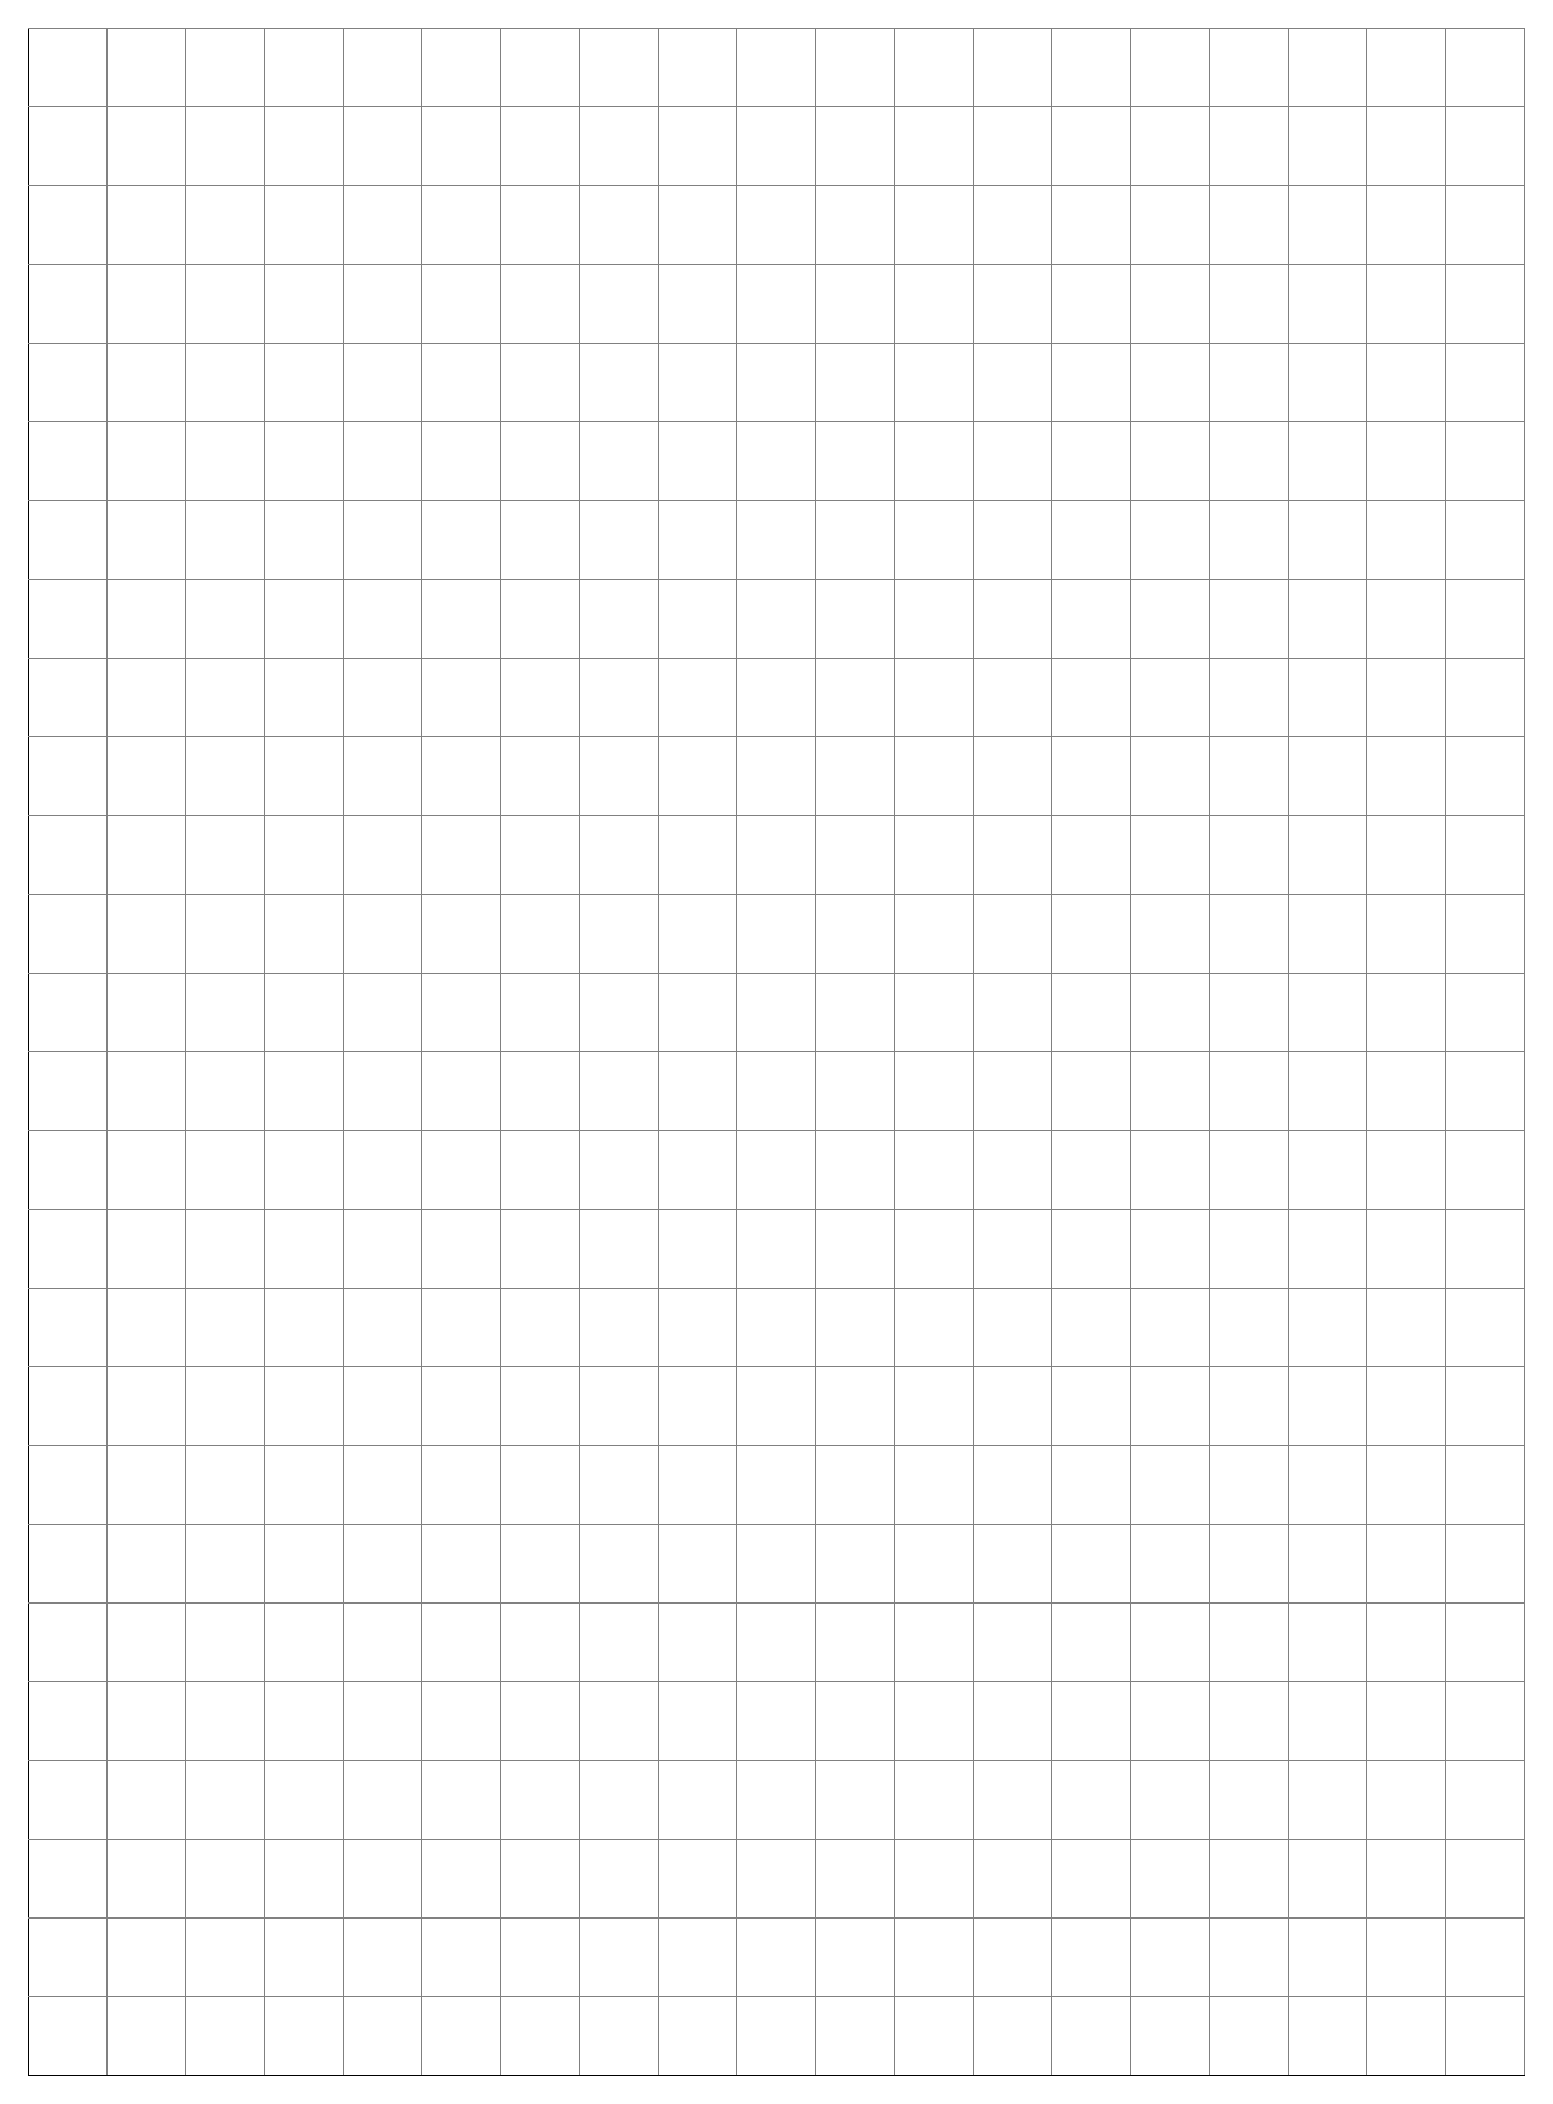
\begin{tikzpicture}
	\draw (0,0)--(19,0)--(19,26)--(0,26)--cycle;
	\foreach \k in {1,...,19}{
		\draw[gray] (\k,0)--(\k,26);	
	}
	\foreach \k in {1,...,26}{
		\draw[gray] (0,\k)--(19,\k);	
	}
	\end{tikzpicture}
\end{figure}
\end{document}
